\documentclass[12pt, a4paper]{article}

\title{\textsc{Linear Algebra} Assignment 3 Report}
\author{110062219 翁君牧}
\date{\today}

\usepackage{xeCJK}
\usepackage{amsmath}
\usepackage{amssymb}
\usepackage{caption}
\usepackage{subcaption}
\usepackage{tikz}
\usepackage{pgfplots}
\usepackage{listings}
\usepackage{hyperref}
\usepackage{booktabs}
\usepackage{biblatex}
\usepackage{longtable}

\lstset{
	breaklines=true,
	basicstyle=\ttfamily,
}

\definecolor{nthu}{HTML}{7F1084}

\begin{document}

\maketitle

\tableofcontents
%\listoffigures

\section{Break the Trajectory into Line Segments}

The route I chose was from my dormitory to a ramen restaurant with 213 track point on the way. I broke the 11 turning points by hands, getting the following results shown in Figure \ref{fig:q1}.

\begin{figure}[htbp]
\centering
\begin{subfigure}{.475\linewidth}
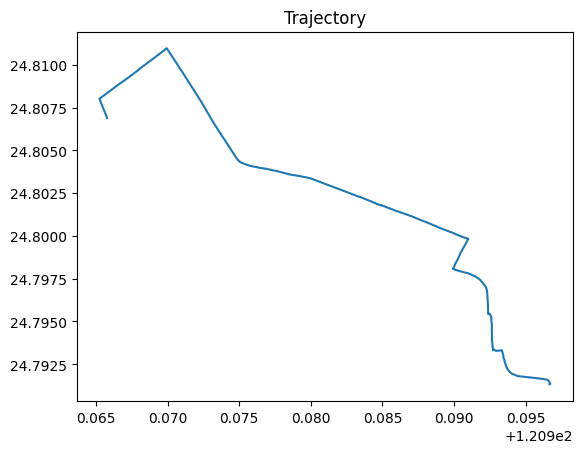
\includegraphics[width=\linewidth]{q1}
\caption{Original}
\end{subfigure}
\begin{subfigure}{.475\linewidth}
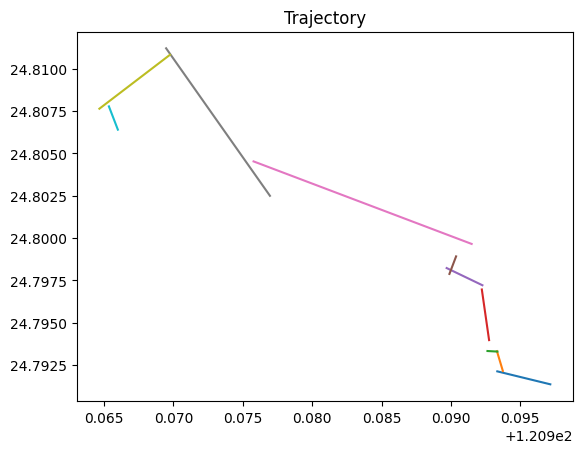
\includegraphics[width=\linewidth]{q1_p}
\caption{Manually broken}
\end{subfigure}
\caption{Trajectory Results}
\label{fig:q1}
\end{figure}

\section{Linear Least Square from \texttt{numpy}}

In the previous assignment, we used \texttt{np.linalg.lstsq()} to solve overdetermined system. This time, we are to perform the linear regression by means of this function.

\subsection{How to know the errors?}

By the documentation, \texttt{np.linalg.lstsq()} computes the approximate solution $\mathbf{x}$ to the system $A\mathbf{x}=\mathbf{b}$ and returns 4 things: the solution $\mathbf{x}$, the \emph{``residuals''}, the rank and the singular values of $A$. The \emph{``residuals''} are defined as ``squared Euclidean 2-norm for each column in $\mathbf{b}-A\mathbf{x}$''. Since we always has $\dim(\mathbf{b})=1$, the first and the only entry of the \emph{``residuals''} is exactly what we want, $||\mathbf{b}-A\mathbf{x}||^2$.

In the notebook, I verified that the \emph{``residuals''} equaled the error for a matrix $A$ of size $1024\times1000$.

\subsection{What's the meaning of \texttt{rcond}?}

Just as I mentioned in the previous report, what \texttt{np.linalg.lstsq()} does is actually to compute the rank and ``pseudo inverse'' of a matrix via singular value decomposition.

So \texttt{rcond} is the threshold rate that if a singular value is less than the largest one, it would be treated as 0 during the process. Since the matrix is always overdetermined, it's pretty fine for us to opt out this feature.

For a matrix $A$ of size $1000\times1024$, I measured the average time of 7 runs (10 loops each), \texttt{rcond} ranging from $10^{-8}$ to $2^{20}\times10^{-8}$. Their time were so close that the difference could be hardly distinguished. Still, the result was plotted in Figure \ref{fig:q2}.

\begin{figure}[htbp]
\centering
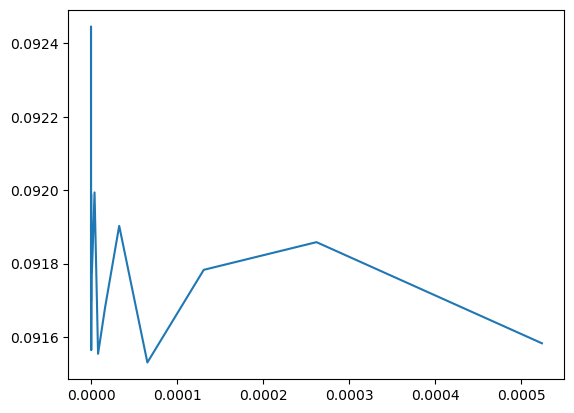
\includegraphics[width=.87\linewidth]{q2}
\caption{Average time w.r.t. \texttt{rcond}}
\label{fig:q2}
\end{figure}

\section{Algorithm that Compresses GPS Data}

My algorithm was described in the 11\textsuperscript{th} cell of the notebook. I maintain the earliest point $p_i$ that is not done yet. For each point $p_j$, if the error of regression segment for $p_i,\dots,p_j$ is greater than $\epsilon$, then $p_j$ should be a turning point.

For the purpose of making all line segments connected, I add additional line segments between the ends.

\begin{figure}[htbp]
\centering
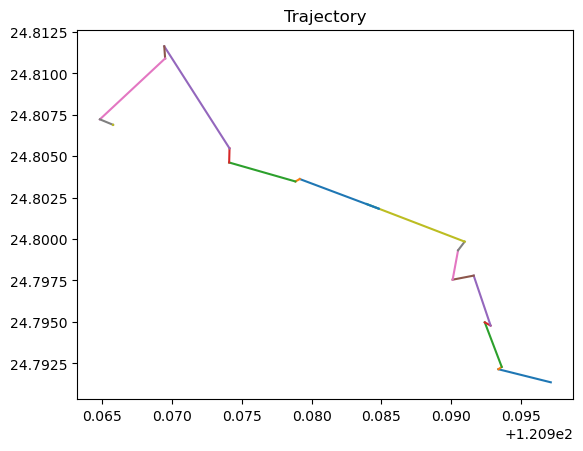
\includegraphics[width=.87\linewidth]{q3}
\caption{Trajectory broken by the algorithm, $\epsilon=3.375\times10^{-6}$}
\label{fig:q3}
\end{figure}

\subsection{Time Complexity}

If there are $m$ points, then $A$ would be of size $m$ by $2$. Thus the time complexity for a \texttt{np.linalg.lstsq()} call would be $O(m\times2^2)=O(m)$.

Generally, \texttt{np.linalg.lstsq()} would be called $O(n)$ times. In the worst case, there would be $O(n)$ points to do regression each time, thus the total time complexity would be $O(n^2)$. In general, if each segment contains at most $m$ points, then the time complexity would be $O(nm)$.

\subsection{Compression Efficiency}

Let's discuss for the specific case, the route provided, the points required with regard to $\epsilon$.

\begin{table}[htp]
\centering
\caption{Compression Efficiency}
\begin{tabular}{lc}
\toprule
$\epsilon$ & \# points \\
\midrule
$10^{-4}$ & 8 \\
$10^{-5}$ & 16 \\
$10^{-6}$ & 39 \\
$10^{-7}$ & 82 \\
\bottomrule
\end{tabular}
\label{tab:q3}
\end{table}

\begin{figure}[htbp]
\centering
\begin{subfigure}{.475\linewidth}
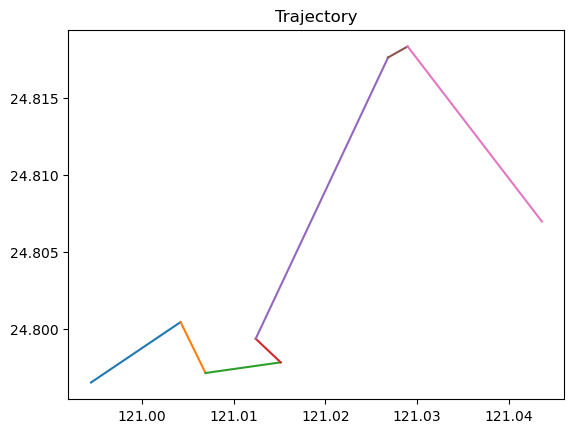
\includegraphics[width=\linewidth]{q3_a}
\caption{$\epsilon=10^{-4}$}
\end{subfigure}
\begin{subfigure}{.475\linewidth}
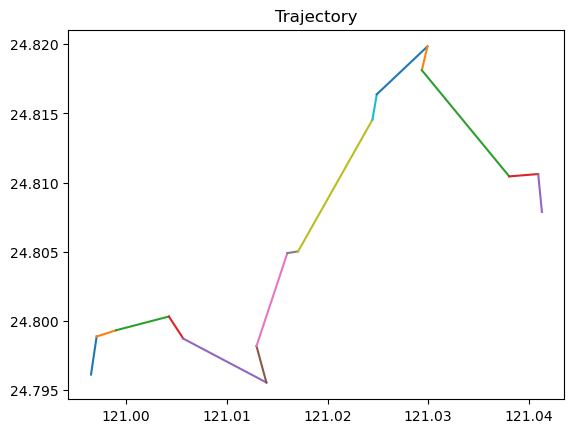
\includegraphics[width=\linewidth]{q3_b}
\caption{$\epsilon=10^{-5}$}
\end{subfigure}
\begin{subfigure}{.475\linewidth}
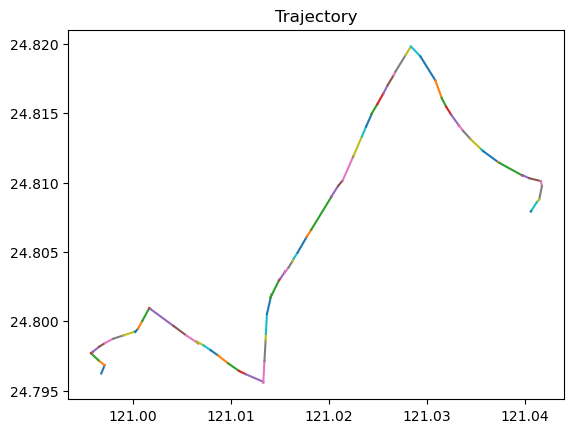
\includegraphics[width=\linewidth]{q3_c}
\caption{$\epsilon=10^{-6}$}
\end{subfigure}
\begin{subfigure}{.475\linewidth}
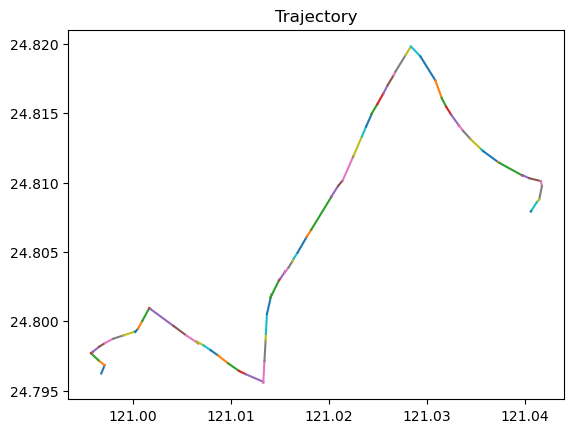
\includegraphics[width=\linewidth]{q3_d}
\caption{$\epsilon=10^{-7}$}
\end{subfigure}
\caption{Trajectory of given route broken by the algorithm}
\label{fig:q3}
\end{figure}

\section{Parabolae Fittings}

The matrix $A$ provided indicates the descending order of coefficients for the linear function. Yet I prefer ascending order so that $A$ would be a \textbf{Vandermonde matrix}.

\subsection{Derivations}

So for the parametric equations of $x,y$, $\left\{\begin{array}{c}x=a_0+a_1t+a_2t^2\\y=b_0+b_1t+b_2t^2\end{array}\right.$, we have the quadratic regression model in this linear system:
$$
A'w'=X-\begin{pmatrix} \epsilon_1 \\ \epsilon_2 \\ \vdots \\ \epsilon_n \end{pmatrix},
A'v'=Y-\begin{pmatrix} \epsilon'_1 \\ \epsilon'_2 \\ \vdots \\ \epsilon'_n \end{pmatrix}
$$, where $A'=\begin{pmatrix} 1 & t_1 & t_1^2 \\ 1 & t_2 & t_2^2 \\ \vdots & \vdots & \vdots \\ 1 & t_n & t_n^2 \\ \end{pmatrix},w'=\begin{pmatrix} a_0 \\ a_1 \\ a_2 \end{pmatrix},v'=\begin{pmatrix} b_0 \\ b_1 \\ b_2 \end{pmatrix}$.

Our goal is to find solutions to $w',v'$ that minimize the error $\sum_{k=1}^n\epsilon_k^2+\sum_{k=1}^n{\epsilon'_k}^2=||A'w'-X||^2+||A'v'-Y||^2$, which is also the sum of square of their 2-dimension norms. Thus we could solve these by \emph{linear least square} again.

\subsection{Curves}

I updated the algorithm to break the trajectory. Yet the function to draw the curves wasn't very well. Maybe I should connect the spaces between parabolae by some straight line segments or smooth curves.

The results are shown in Figure \ref{fig:q4} \& \ref{fig:q4_p}.

\begin{figure}[htbp]
\centering
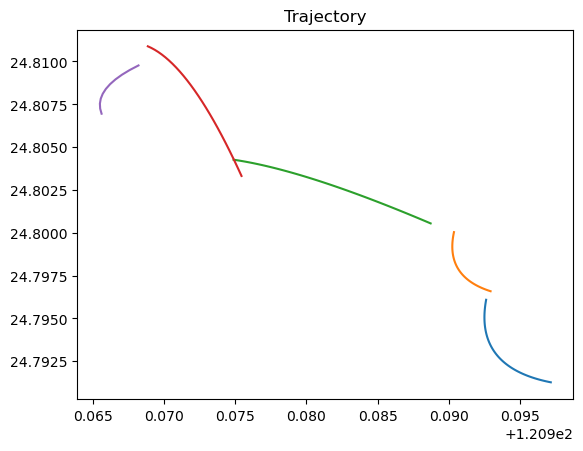
\includegraphics[width=.69\linewidth]{q4}
\caption{Parabola fitting of my route with $\epsilon=10^{-5}$}
\label{fig:q4}
\end{figure}

\begin{figure}[htbp]
\centering
\begin{subfigure}{.45\linewidth}
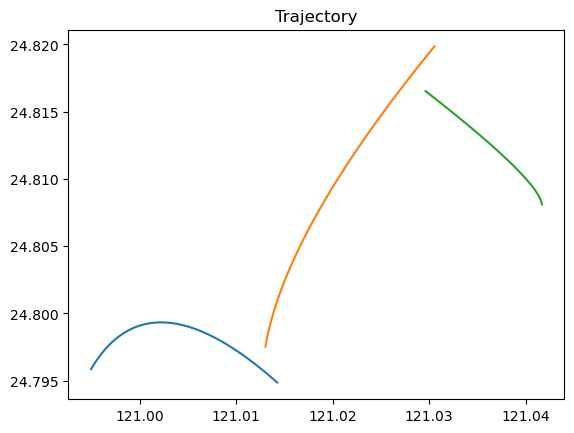
\includegraphics[width=\linewidth]{q4_a}
\caption{$\epsilon=10^{-4}$}
\end{subfigure}
\begin{subfigure}{.45\linewidth}
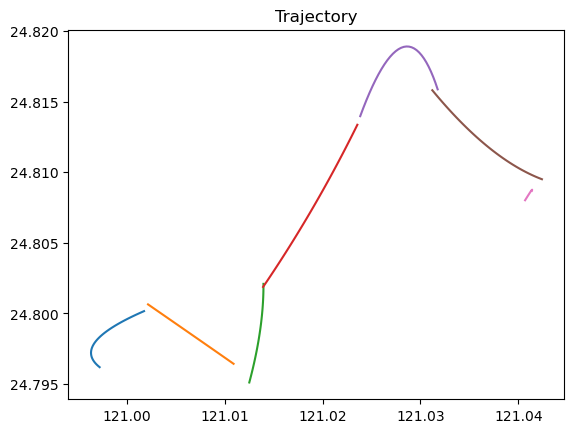
\includegraphics[width=\linewidth]{q4_b}
\caption{$\epsilon=10^{-5}$}
\end{subfigure}
\begin{subfigure}{.45\linewidth}
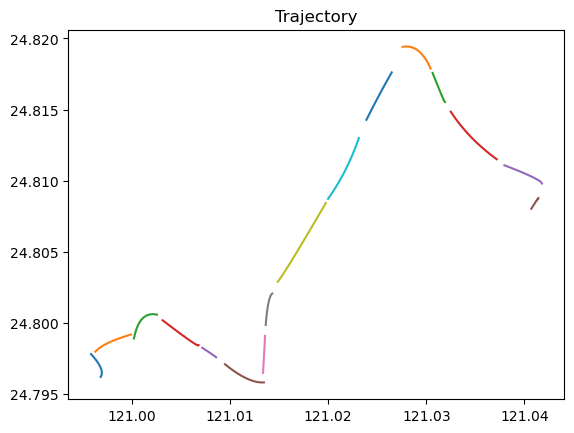
\includegraphics[width=\linewidth]{q4_c}
\caption{$\epsilon=10^{-6}$}
\end{subfigure}
\begin{subfigure}{.45\linewidth}
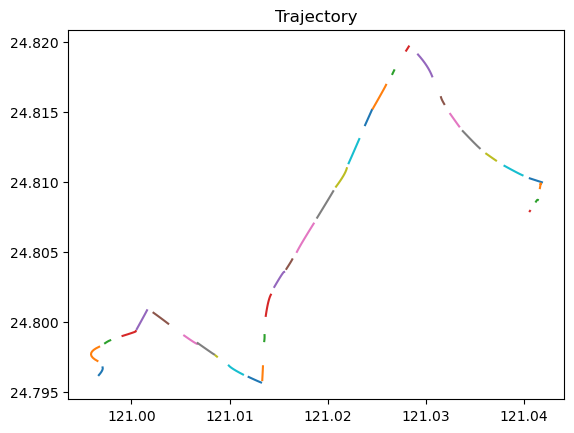
\includegraphics[width=\linewidth]{q4_d}
\caption{$\epsilon=10^{-7}$}
\end{subfigure}
\caption{Parabolae fittings of given route with different $\epsilon$}
\label{fig:q4_p}
\end{figure}

\section{Total Least Square}

There are various sort of \emph{linear least squares}. The most common one, \emph{ordinary least squares}, is aimed at finding a regressive line to predict the response variables. As a consequence, it only consider the distance in $y$-axis.

On the other hand, \emph{total least squares}, a generalization of \textbf{orthogonal regression}, takes the errors for covariate variables into account. That is, our objective is to find a regressive line that the orthogonal distances between all points and the line is minimized.

\texttt{scipy} provides a module that dedicates to perform the \textbf{orthogonal distance regression}. There are inbuilt linear, quadratic, exponential models. Yet I tried linear one only.

We could see that in Figure \ref{fig:q5}, if we take $\epsilon\leq10^{-5}$, then the results of \emph{OLS} and \emph{ODR} are almost the same; when $\epsilon\geq10^{-6}$, their difference are not distinguishable at the first glance.

\begin{figure}[htbp]
\centering
\begin{subfigure}{.475\linewidth}
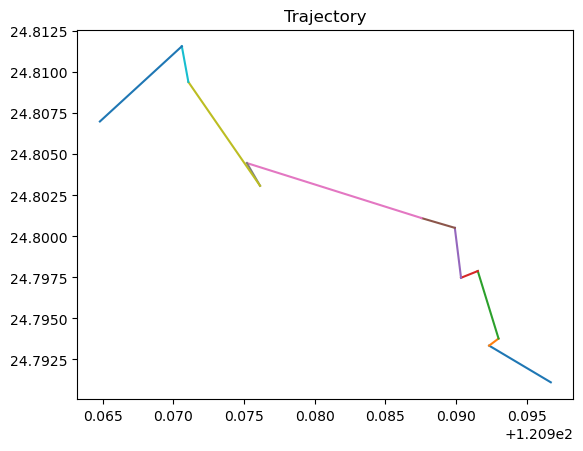
\includegraphics[width=\linewidth]{q5}
\caption{$\epsilon=10^{-6}$}
\end{subfigure}
\begin{subfigure}{.475\linewidth}
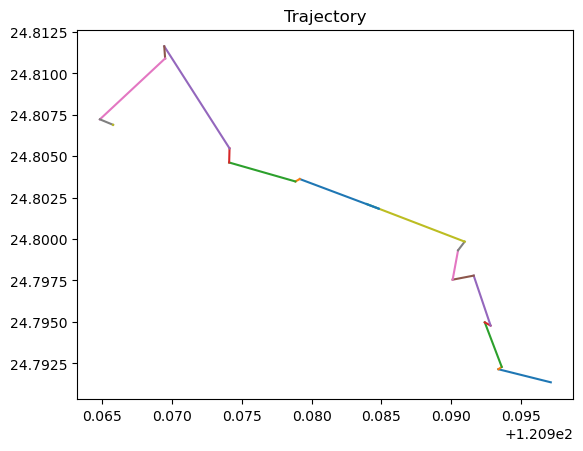
\includegraphics[width=\linewidth]{q5_p}
\caption{$\epsilon=3.375\times10^{-6}$}
\end{subfigure}
\caption{ODR of my route}
\end{figure}

\begin{figure}[h]
\centering
\begin{subfigure}{.45\linewidth}
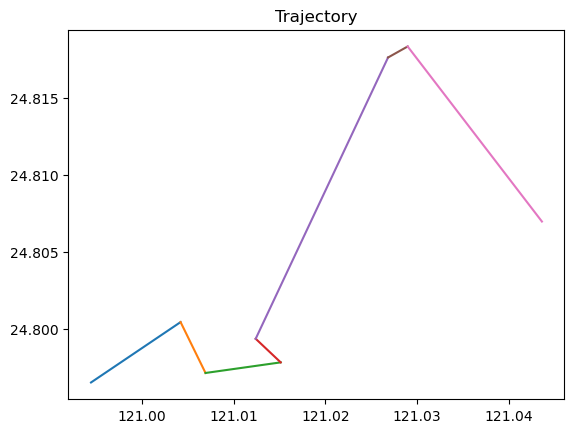
\includegraphics[width=\linewidth]{q5_a}
\caption{$\epsilon=10^{-4}$}
\end{subfigure}
\begin{subfigure}{.45\linewidth}
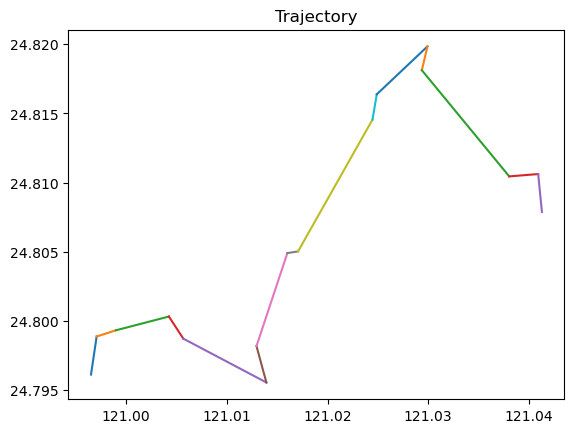
\includegraphics[width=\linewidth]{q5_b}
\caption{$\epsilon=10^{-5}$}
\end{subfigure}
\begin{subfigure}{.45\linewidth}
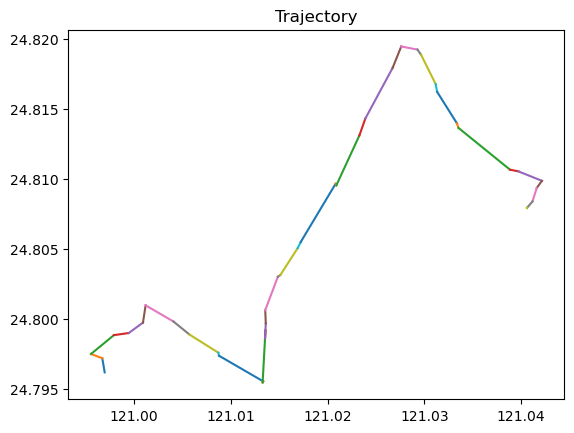
\includegraphics[width=\linewidth]{q5_c}
\caption{$\epsilon=10^{-6}$}
\end{subfigure}
\begin{subfigure}{.45\linewidth}
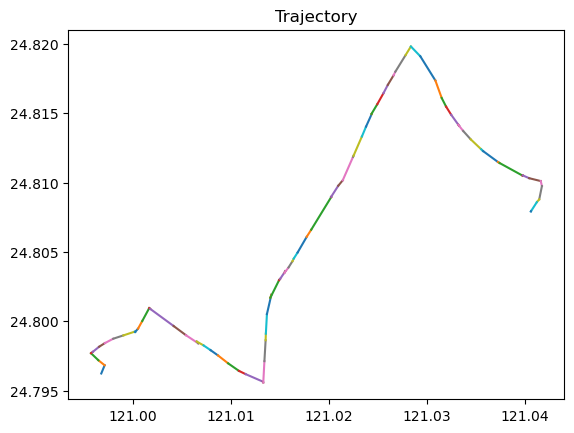
\includegraphics[width=\linewidth]{q5_d}
\caption{$\epsilon=10^{-7}$}
\end{subfigure}
\caption{ODR of given route with different $\epsilon$}
\label{fig:q5}
\end{figure}

\pagebreak[4]

\section*{Acknowledgements}

I thank to \textsf{National Center for High-performance Computing} \textit{(NCHC)} for providing computational and storage resources.

\end{document}
